Error-resilience is typically a topic discussed orthogonally to congestion
control, mainly because error-resilience caters to handling
packet loss while congestion control caters to the amount of information sent
over the network. This chapter is based on our work on unifying
error-resilience and congestion control.

In \citepub{c:err}, we evaluate the performance of the various
error-resilience schemes available for use in interactive multimedia
communication (mainly applicable to H.264). These are: using Negative
Acknowledgement (NACK) or Packet Loss Indication (PLI), Forward Error
Correction (FEC) or Unequal Level of Protection (ULP), adaptive slice sizes,
and Reference Pictures Selection Indication (RPSI). We evaluate the
performance of the proposed mechanisms in diverse scenarios in a simulated
environment (in ns-2) using real-world 3G loss patterns~\cite{3gppSim}.
Lastly, based on our observations, we define the applicability of the various
error-resilience with respect to end-to-end latency and packet loss.

In \citepub{c:fecrc}, we propose using FEC not only for error-resilience but
also for congestion control, i.e., instead of probing for available capacity
by increasing the sending rate of the media stream, the endpoint sends
redundant packets. If a packet gets lost and the added FEC packet arrives in
time, the receiving endpoint would recover the lost packet. However, if the
packet is not lost, by introducing the FEC packet the sender not only
discovers that there is additional available capacity, but also has a sense of
the (minimum) magnitude of the available capacity. We compare our proposal
with our previous work in \citepub{c:3grc} and \citepub{c:hetrc}, and 
RRTCC~\cite{draft.rrtcc}. We evaluate the performance of the
mechanisms in diverse scenarios implemented in a simulation environment (in
ns-2) and in our testbed.

\section{Error-resilience Schemes}
% explain all 4 and the adaptivity

H.264~\cite{h264} uses various error-control methods~\cite{err_res_h264_std,
wang98error, wang00review, 310669} to overcome loss due to corruption (e.g.,
in wireless) and non-bursty packet loss (e.g., due to congestion). These
methods are classified into three categories: source coding, channel coding,
and joint source and channel methods. Source coding refers to the methods
implemented by the video codec. Channel coding refers to the methods
implemented by the networking layer. Joint source-channel refers to methods
that combine source-coding and network-coding mechanisms.

The H.264/AVC codec has several features that support error-resilient
mechanisms for video communication that correspond to the above
categorization~\cite{310669}. At the codec level, the following are available:
adaptive slice size, Reference Picture Selection (RPS), and Flexible
Macroblock Ordering (FMO)~\cite{err_res_h264_std, wenger_ott_jscc}. Similarly,
at the channel level, the following are available: Selective Retransmission
(NACK), and PLI. An example of joint source-channel is UEP with 
FEC~\cite{wang00review}, in which the sender
attempts to selectively protect important parts of the bitstream or 
encodes redundant frames differently than other frames~\cite{ervcuupkp}.
% pictures -> frames

The performance of the available error-resilience mechanisms vary with the
observed end-to-end latency, link loss, bandwidth constraints and operating
environment (3G/LTE to 3G/LTE, 3G/LTE to WLAN, or wireless to fixed, etc.). No
single error repair mechanism fits all operating environments. A solution that
works for an observed packet loss ratio of less than 2\,\%, may not scale well
for paths with higher packet loss or higher latency.

% The combination of end-to-end delay requirements, capacity constraints and
% varying packet loss rate require different error resilience mechanisms.

\begin{figure}
\centerline {
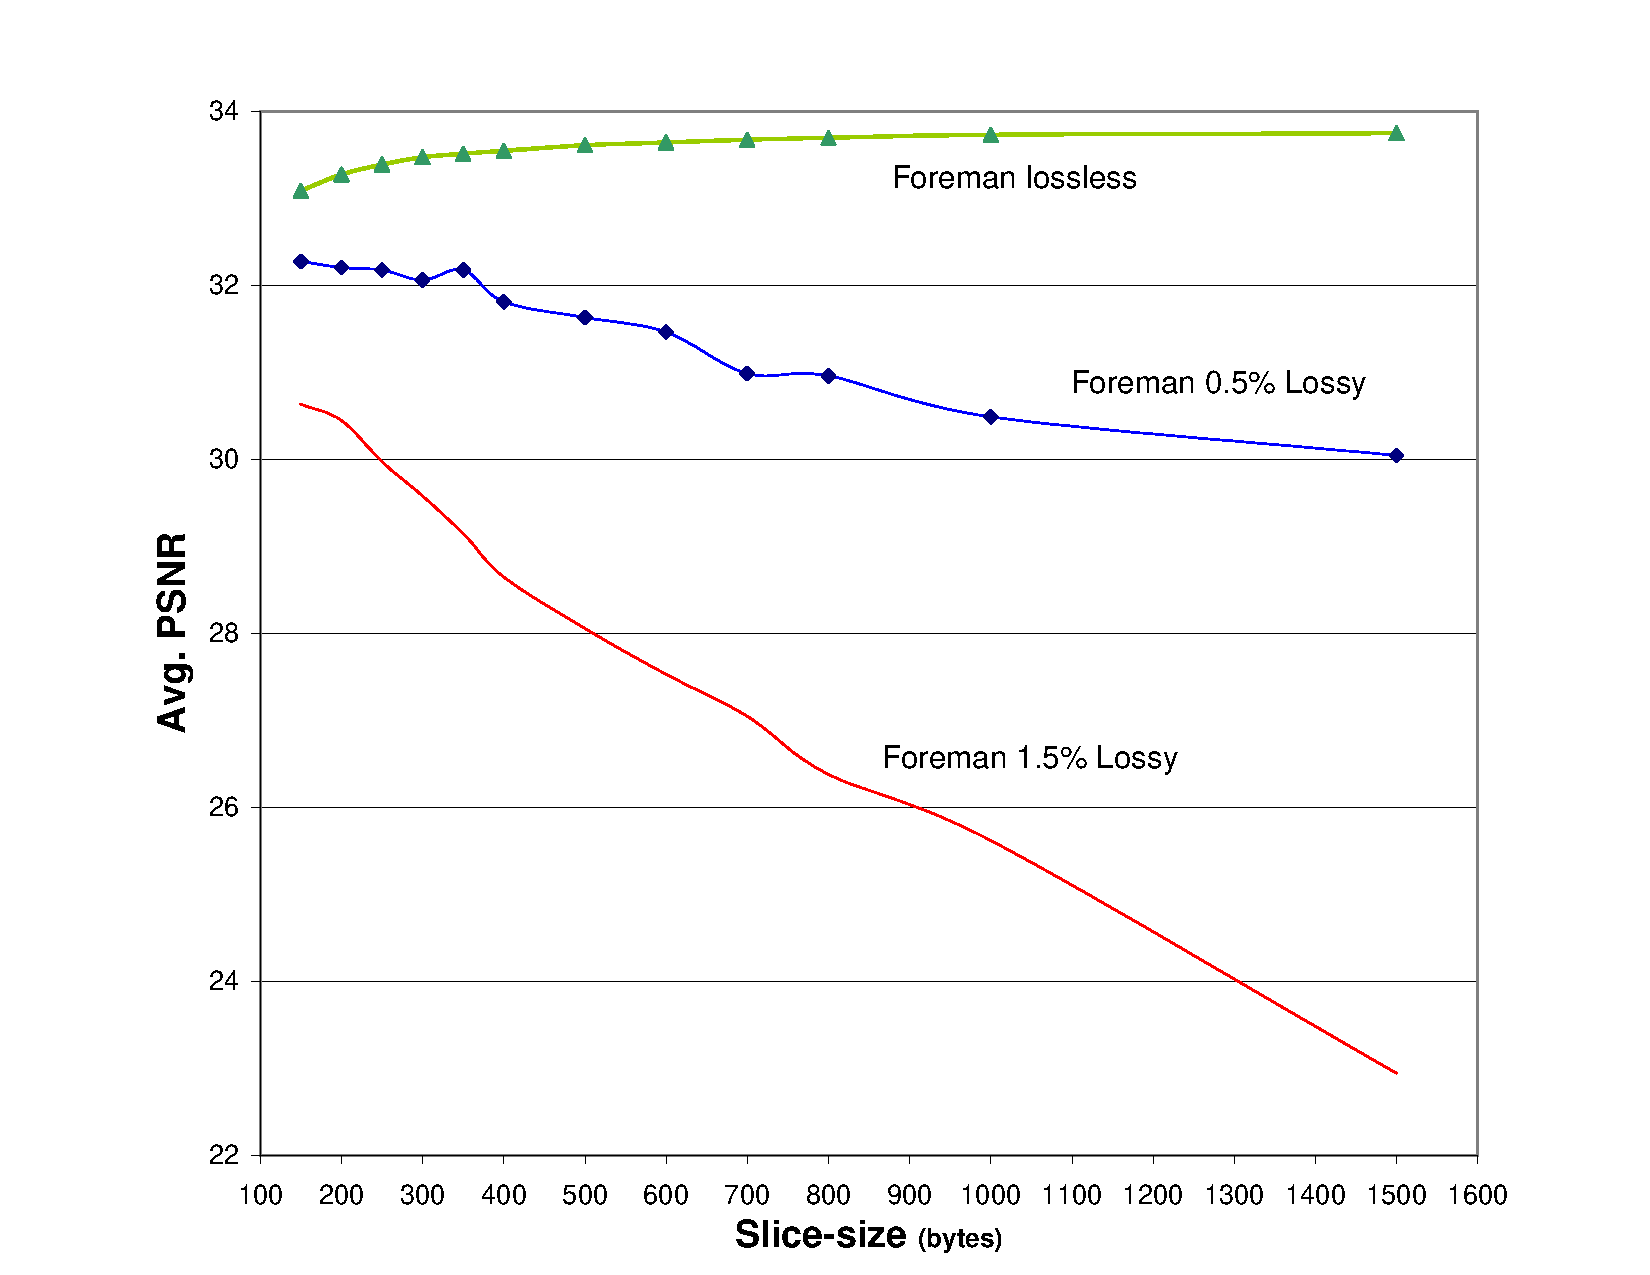
\includegraphics[width=0.66\textwidth]{chap6-graph-slicesize_mot}
}
\caption{Effect of different slice sizes on PSNR for links experiencing different amounts of bit-error corruption.}
\label{fig:slicesize_mot}
\end{figure}

\begin{itemize}
\setlength{\itemsep}{0pt}

  \item \textbf{\texttt{Retransmissions}}: In RTP, retransmissions are either
  payload-specific or at the transport-specific. Transport-specific loss
  contains packet loss information (Generic NACK), while payload-specific loss
  contains Slice Loss Information (SLI), Picture Loss Information (PLI) or
  Reference Picture Selection indication (RPS). Typically, the receiver
  detects a loss and sends it as soon as the RTCP reporting interval allows
  feedback.

  \item \textbf{\texttt{Adapting Slice Sizes}}: the encoder adapts the size of
  the picture slice based on the link characteristics; when the channel is
  lossless there can be one picture per slice (up to the MTU size) and when
  high losses are reported, the slices are reduced in size (up to 100 bytes).
  Larger slice sizes improve encoding efficiency, but are more vulnerable to
  frame losses. Figure~\ref{fig:slicesize_mot} shows the variation of average
  PSNR with respect to different slice sizes in varying loss scenarios. We
  observe that there is a direct correlation between packet loss, slice
  size and media quality.

  \item \textbf{\texttt{Reference Picture Selection}}: Instead of
  retransmitting a lost packet, the encoder finds the list of correctly
  received pictures (or frames) by the decoder. Hence, for subsequent encodings, the
  encoder uses a different decoded picture for inter-prediction reference.
  This method stops the temporal error propagation caused by an earlier packet
  loss. In the RPS message, the decoder reports the list of pictures (or frames)
  that were correctly received or lost. Hence, the encoder is able to retrieve
  the lost picture data. The mode of operation can be decided
  depending on the observed packet loss rate.

  \item \textbf{\texttt{Unequal Error Protection}}: When the link latency is
  high, retransmissions cannot be used because the
  retransmitted packets arrive too late to be played back. In these cases, the
  sender proactively uses a portion of the available capacity to send
  redundant packets (typically, FEC), hoping to recover any lost packet before
  decoding. Hence, by using UEP, the media senders try to strike a balance by
  protecting only a chosen set of the media packets. In \citepub{c:err}, we
  protect the reference frames and not the non-reference frames with UEP.

\end{itemize}

In \citepub{c:err}, we stream three different YUV sequences~\cite{YUV_seq} over a
3G link simulated in \emph{ns-2}~\cite{ns2} with varying amount of link layer
packet loss (0.5\,\%, 1.0\,\% and 1.5\,\%)~\cite{3gppSim}. Our experiments
show that using NACK, the endpoint is able to correct 15-30\,\% of the lost
packets for an end-to-end path latency of 60\,\emph{ms}, which meets the
preferred  packet latency of 150\,\emph{ms} specified by ETSI~\cite{etsi.qoe}.
The number of recovered packets will increase with shorter RTCP reporting
intervals; in this paper, we use a 1\,\emph{s} reporting interval, with early and
immediate reporting as defined in \cite{rfc4585}. Our experiments show that
NACK is an effective mechanism for low delay scenarios. Similarly, protecting
the media flows with UEP incurred a 15-25\,\% overhead, and about 21-24\,\% of
the lost packets were recovered.

\begin{figure}
\centerline {
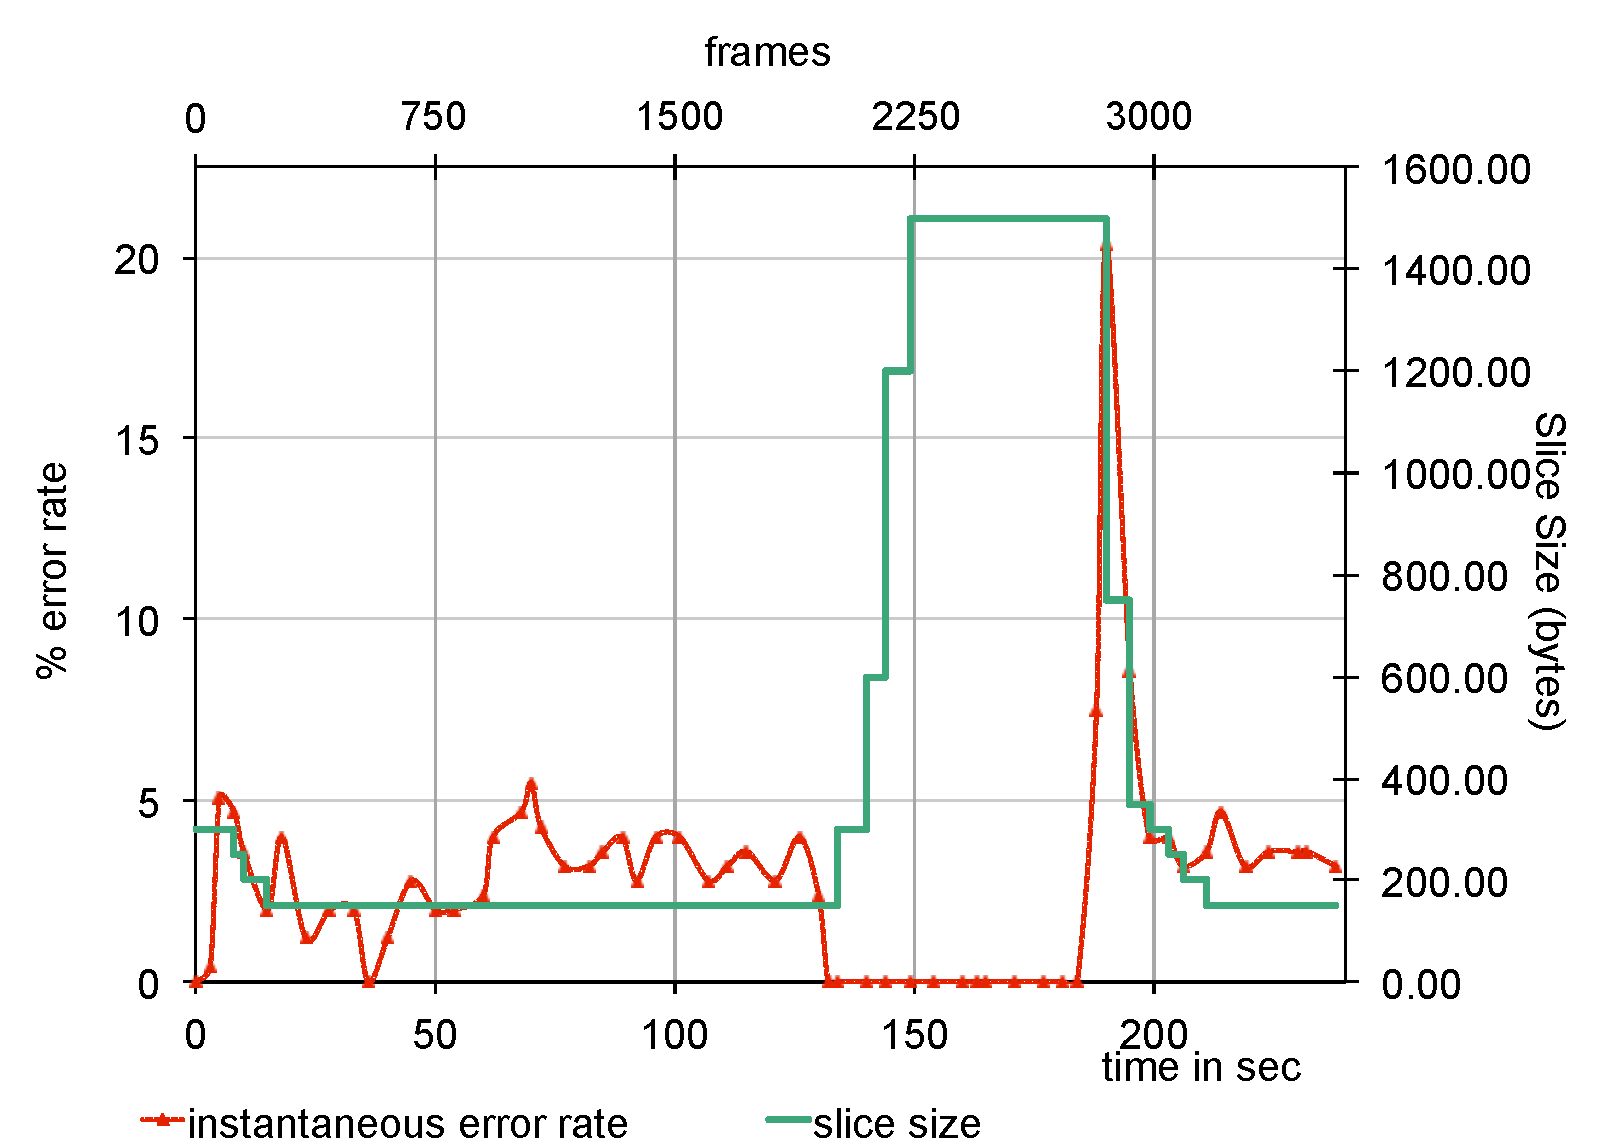
\includegraphics[width=0.66\textwidth, 
    clip=true, trim=0cm 0cm 0cm 2.5cm]{chap6-graph-ssa_adapt}
}
\caption{The plot shows the variation in slice sizes with varying error
rates.}
\label{fig:ssa_adapt}
\end{figure}

Senders use a moving average of the last three observed fraction loss rates
reported in the RTCP RR to vary the slice size. The slice size is doubled for
every period with average loss below 1.0\,\% until it reaches the MTU size
(1500 bytes). Slice sizes remain constant for loss rates between 1\,\% to
2.5\,\% to provide stability to the receiving system. However, in high loss
scenarios, if the slice size is larger than 400 bytes, it is halved, and for
sizes below 400 bytes, it is reduced in steps of 50 bytes to a minimum of 150
bytes. Figure ~\ref{fig:ssa_adapt} shows variation of slice-size with the
instantaneous loss rate and the average loss rate. Hence, by adapting the
slice sizes, the sender is not repairing the stream (or replacing the missing
packets), rather, it is attempting to constrain the area of errors in the
picture. If an RTP packet containing a small-sized slice is lost, a smaller
area of the decoded picture is affected, alternatively, when a packet
containing a large-sized slice is lost, a large part of the decoded picture 
or the complete picture is affected.

Lastly, using the RPS error-resilience mechanism, the receiver indicates the
decoding correctness when losses occur, i.e., which pictures or slices have
been decoded correctly or incorrectly.  In our experiments, the receiver sends
RTCP RR every 250\,\emph{ms}, which increases the reporting overhead to 2\,\%
of the session bandwidth. In Figure ~\ref{fig:rpsi_sim} (a), (b) and (c), we
observe that the PSNR drops down when a lost frame is referenced and the PSNR
increases immediately after the encoder chooses a correct reference picture.
When the one-way latency is 100\,\emph{ms} and the frame rate is set to 15
frames per second, we observe that the error propagation is stopped by RPS in about
4 to 7 picture frames.


\begin{figure}[!t]
  \centering{
  \subfloat [Foreman]{
    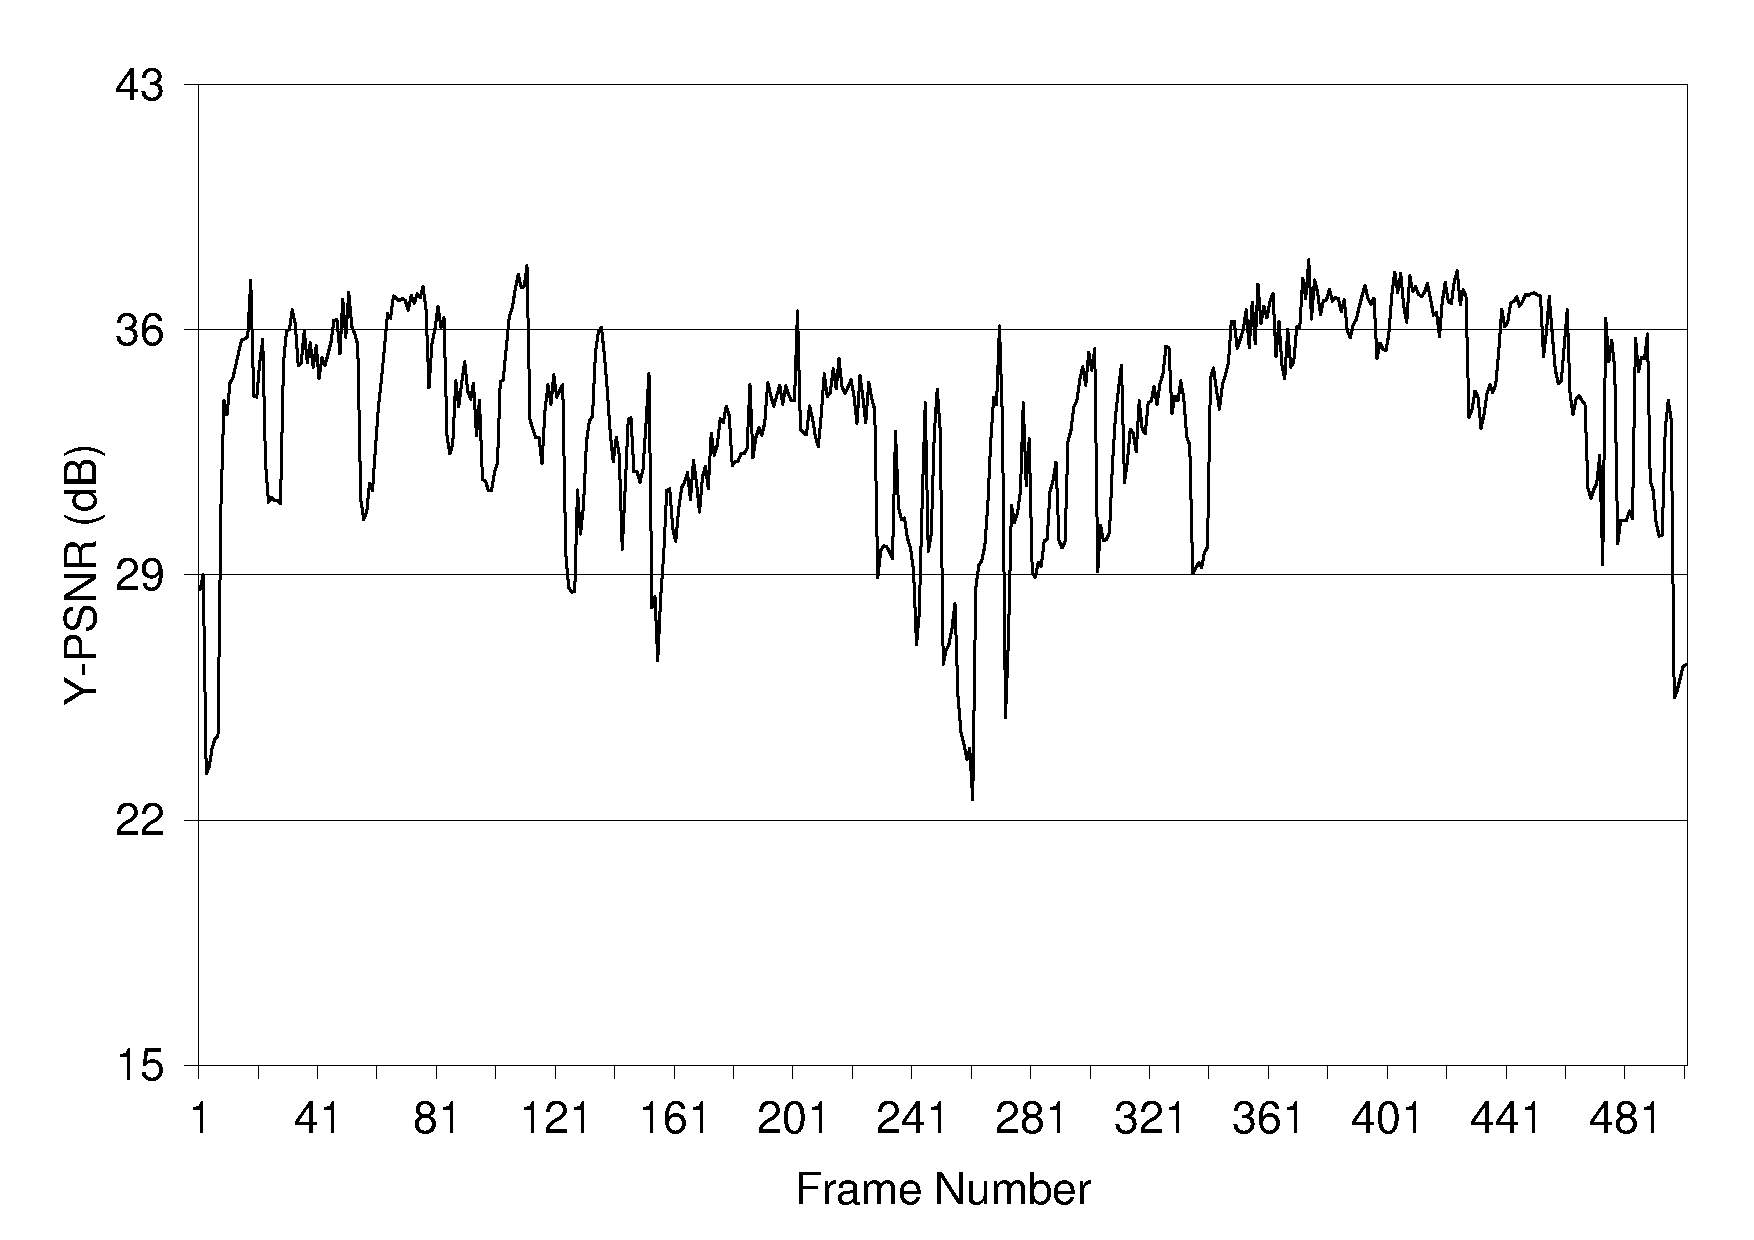
\includegraphics[width=0.5\textwidth]{chap6-graph-rpsi-1}
  } \\
  \subfloat [News]{
    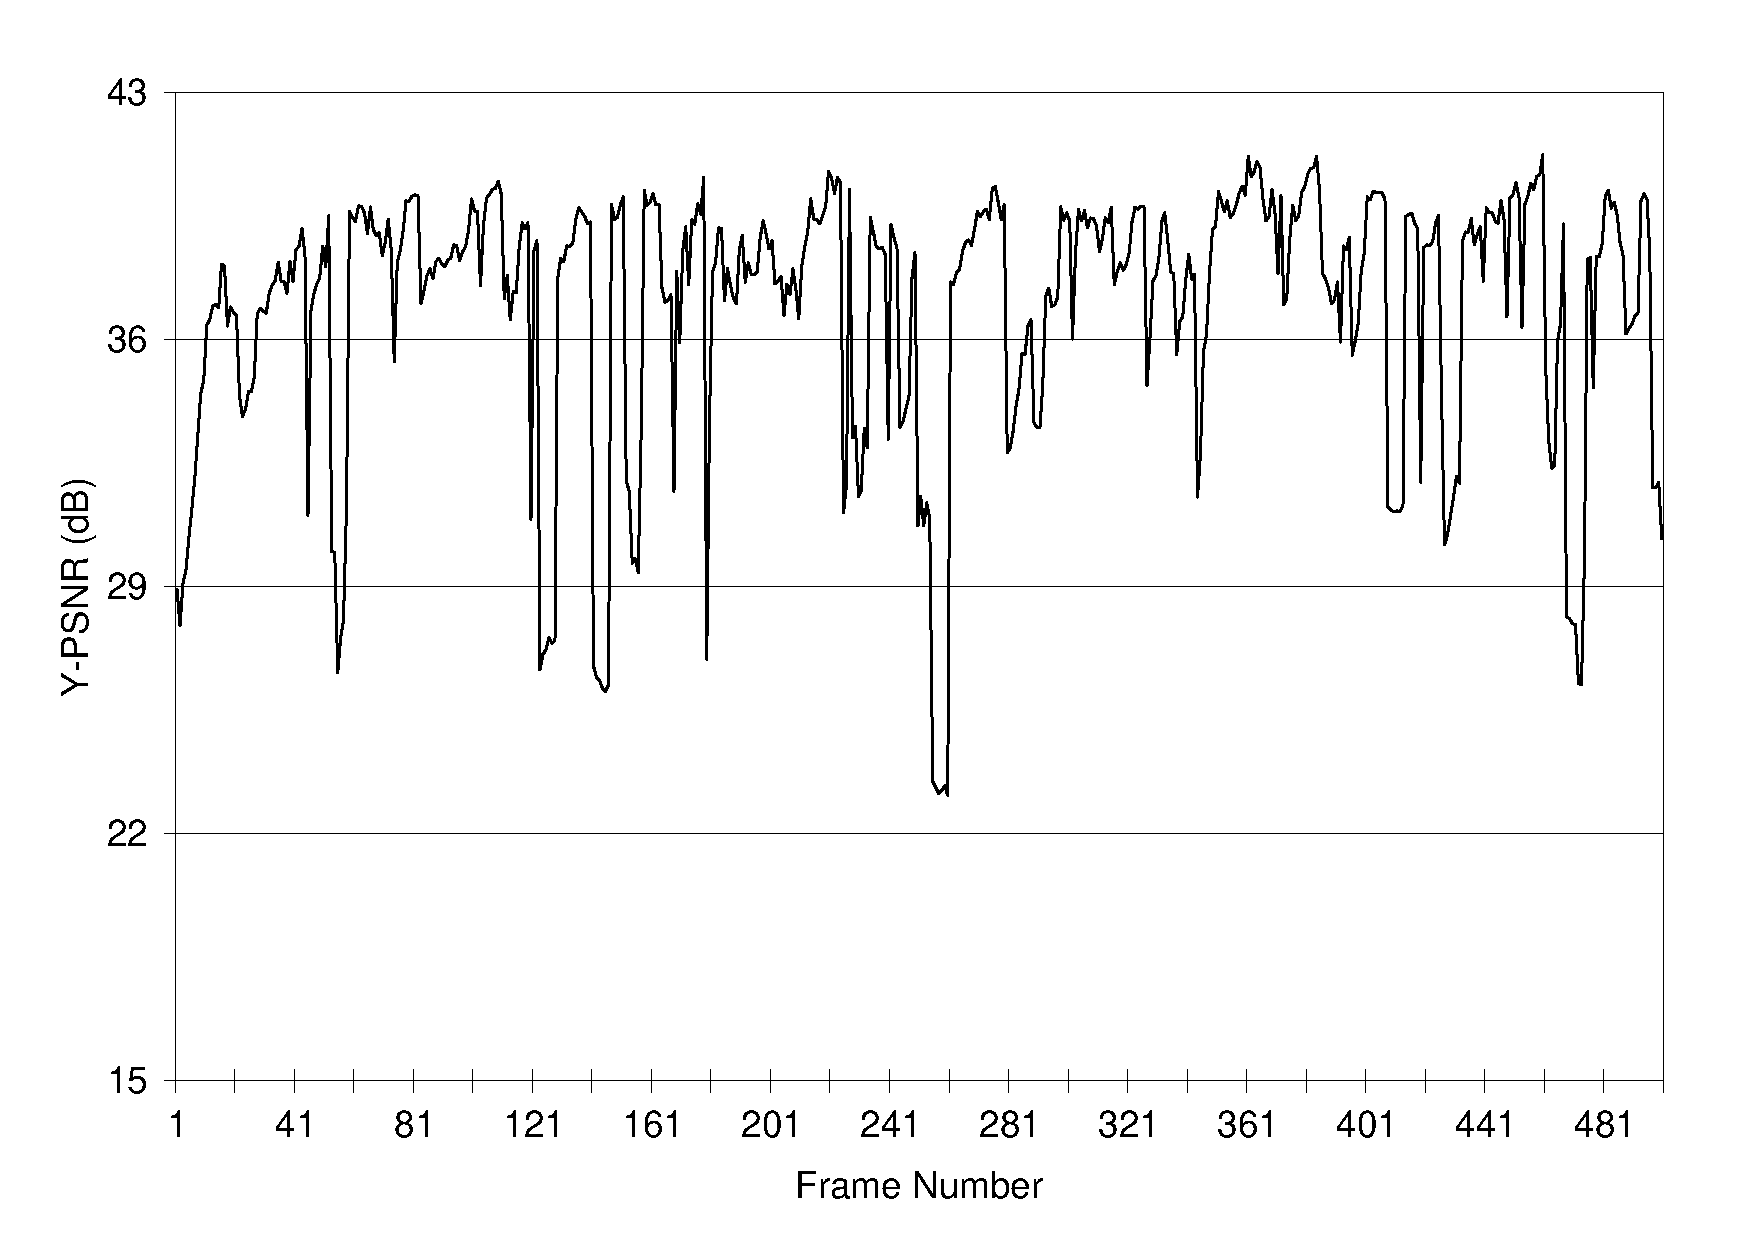
\includegraphics[width=0.5\textwidth]{chap6-graph-rpsi-3}
  } \\
  \subfloat [Football]{
    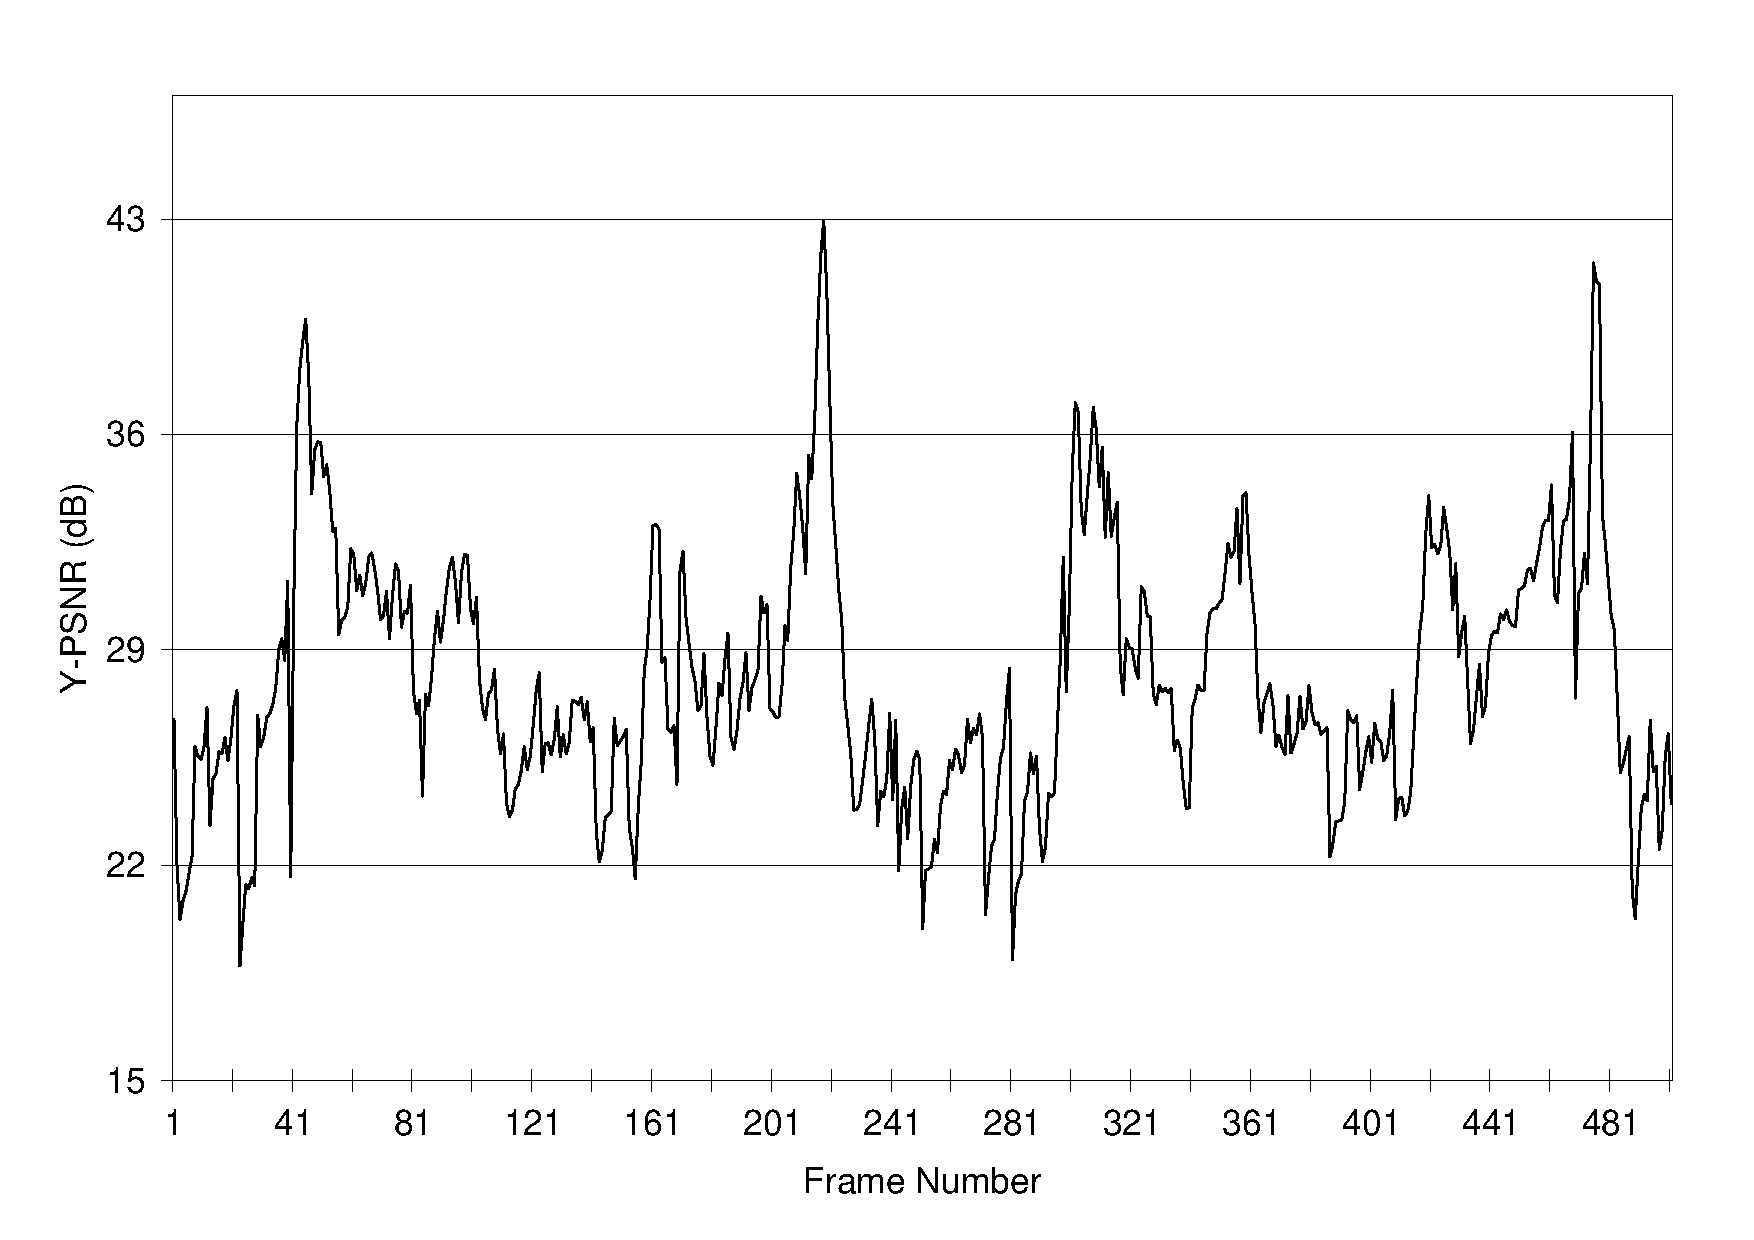
\includegraphics[width=0.5\textwidth]{chap6-graph-rpsi-5}
  }
}
\caption{The plots show the PSNR variation when using RPSI to stop decoding
error propagation for (a) Foreman, (b) News, and (c) Football sequences.}
\label{fig:rpsi_sim}
\end{figure}

Table~\ref{tab:err-sch-psnr} presents the average PSNR of the different 
error-resilience schemes for links with 0.5\,\% fractional loss. We observe that the
RPS performs better than UEP and NACK and is comparable to adaptive slices.
The UEP underperforms mainly because the media stream is encoded at a lower
rate to make room for FEC, compared to the media streams of the other
error-resilience mechanisms.

\begin{table}
  \centering{
  \scalebox{0.75}{
\begin{tabular}{cccc}
\hline
 & \multicolumn{3}{l}{Y-PSNR, 0.5\,\% PLR} \\
\hline
 & Foreman & Football & News  \\ \hline
NACK & 32.1456 & 28.0331 & 35.3867 \\
RPSI & 33.68 & 28.05 & 37.37 \\
UEP & 28.33 & 26.86 & 34.47 \\
Adaptive slices & 32.30 & 28.4 & 37.25 \\
\hline
\end{tabular}
}}
\caption{Comparing the performance of different error-resilience
schemes on three different types of YUV sequences~\cite{YUV_seq}. The link
loss rate is 0.5\,\% at each 3G link.}
\label{tab:err-sch-psnr}
\end{table}

In \citepub{c:err}, we model the error-resilience mechanisms as a function of
observed packet loss and end-to-end delay (or latency), and
Figure~\ref{fig:apply_err} summarizes the applicability of the
error-resilience mechanisms based on our experiments. NACK is useful when loss
rates are low and the end-to-end delay is also low. Adaptive slice size (SSA)
is applicable to the whole operational region because it attempts to scale the
packet size based on the observed loss rate, but does not help in packet
repair. RPS works better on links with bursty packet loss, where NACK would
not be effective. By correctly choosing a new reference picture, the sender is
more effective when network latency is higher. UEP/FEC schemes are mainly useful when
the sender and receiver cannot effectively co-operate to repair the stream and
the fractional loss is within the FEC's chosen protection range.

\begin{figure}
\centerline {
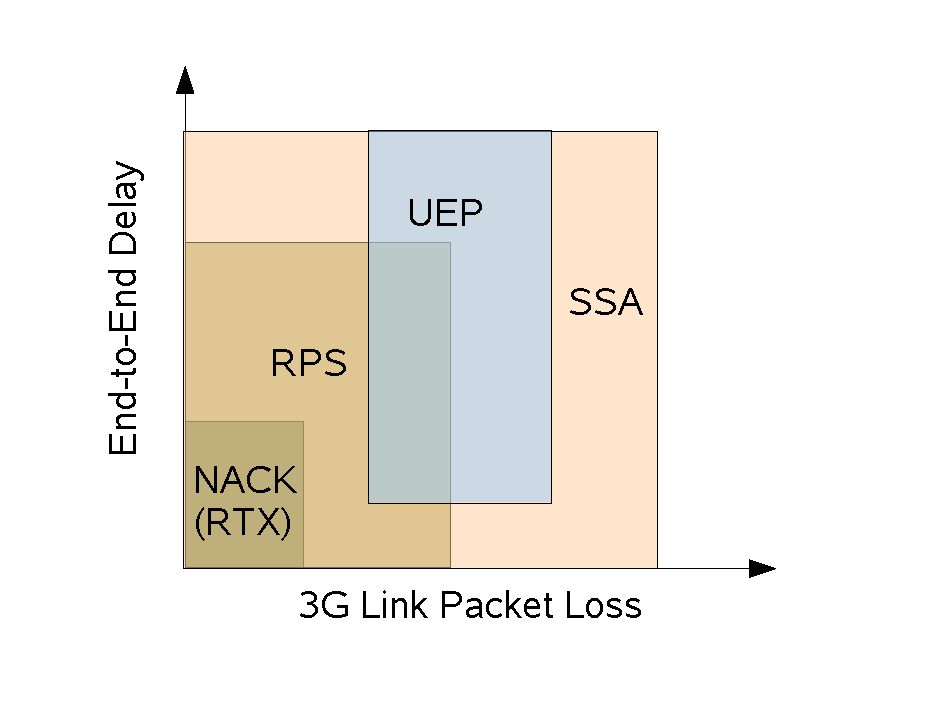
\includegraphics[width=0.75\textwidth, 
    clip=true, trim=0cm 1cm 0cm 1cm]{chap6-fig-apply-err}
}
\caption{Applicability of the error-resilience schemes in a heterogeneous
environment containing both wireless and wired links.}
\label{fig:apply_err}
\end{figure}


\section{Using FEC for Congestion Control}

For many years, conversational multimedia flows have used FEC for error 
protection~\cite{855913, 664283}, i.e., the
application trades off additional sending rate for redundant packets to reduce
the effect of losses. In \citepub{c:err}, we show that 21-24\,\% of the lost
packets are recovered using a static amount of FEC. In \citepub{c:fecrc}, we
investigate the use of FEC packets not only for error-resilience but also as a
probing mechanism for congestion control.

Zhu~\textit{et al.}\cite{Zhu:2001tu,springerlink:1022865704606} propose using
ULP for both congestion control and error-resilience. 
Firstly, they estimate the available rate using a variant of TFRC,
called Multimedia Streaming TCP-Friendly Protocol (MSTFP)~\cite{871542}.
Secondly, they take packet loss and historical sending rate to smooth out the
encoding rate. Lastly, they apply FEC while performing congestion control and
their results show a significant increase in media quality. MSTFP, on the other
hand, does not use RTP/RTCP and acknowledges each packet for calculating the
TFRC estimate.


\begin{figure}
  \centering
  \subfloat [Concept]{
    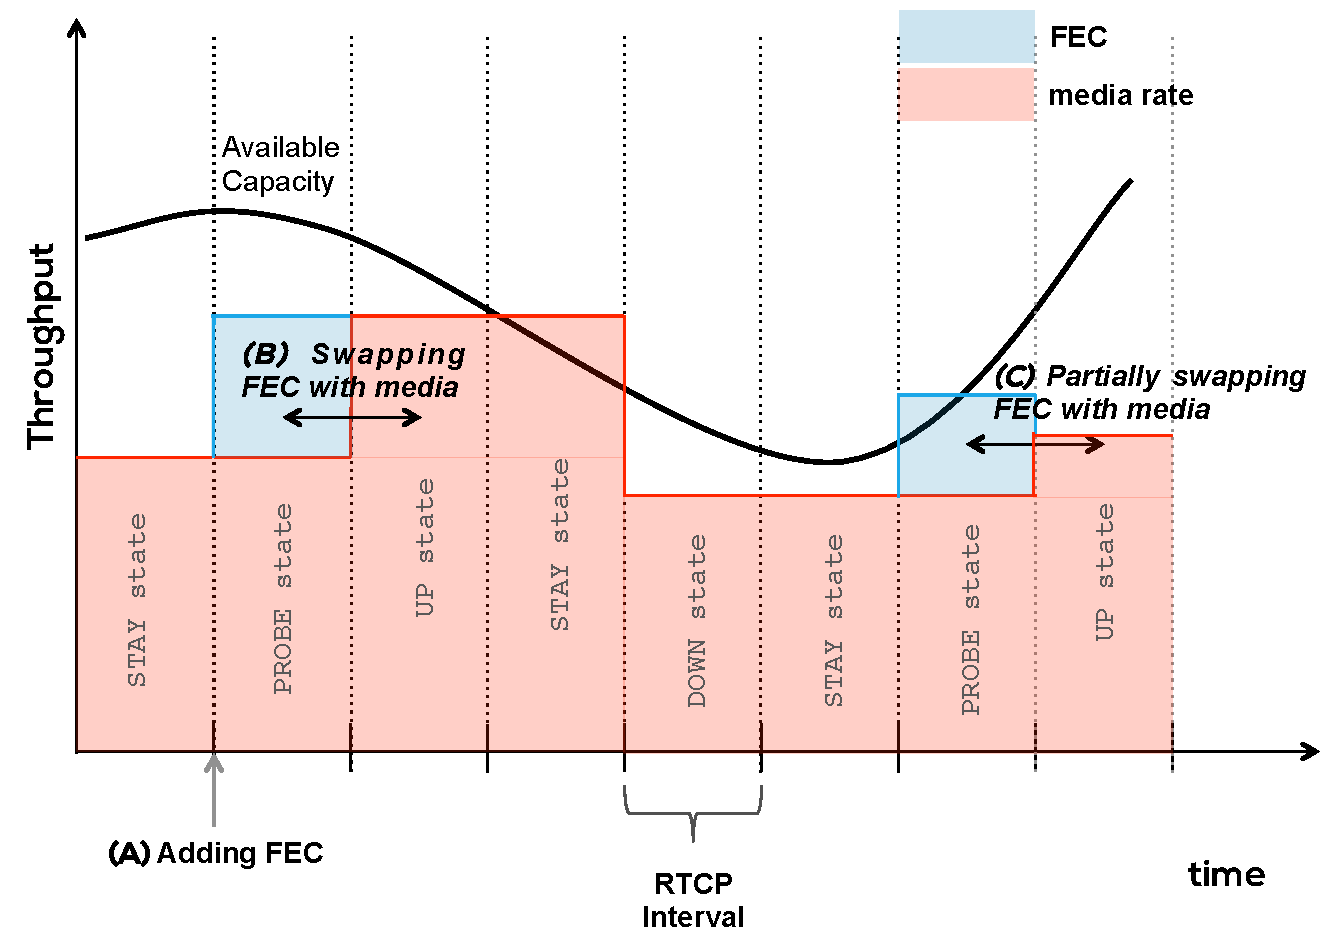
\includegraphics[width=0.66\textwidth]{chap6-fig-fecrc-concept}
  } \\
  \subfloat [State-machine]{
    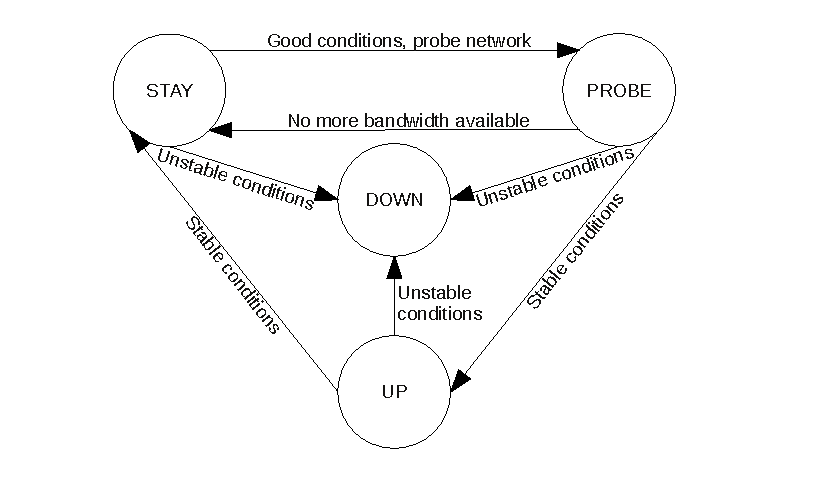
\includegraphics[width=0.66\textwidth]{chap6-fig-fecrc-state}
  }
\caption{a) Interaction of FEC and congestion control, b) FEC-Based Rate
Adaptation (FBRA) state machine.}
\label{fig:fecrc-intro}
\end{figure}

Our concept in \citepub{c:err} is similar to that described in
\cite{Zhu:2001tu} but applied to interactive multimedia. The concept is as
follows: the sender chooses a high FEC rate to aggressively probe for
available capacity and conversely chooses a low FEC rate to conservatively
probe for available capacity. While probing, if a packet is lost and the FEC
packet arrives in time for decoding, the receiver is be able to recover the
lost packet; if no packet is lost, the sender is able to increase the media
encoding rate by swapping out the FEC. Figure~\ref{fig:fecrc-intro}(a) shows
the endpoint adding FEC and then swapping it for additional media. This method
can be especially useful when the sending rate is close to the bottleneck link
rate: by choosing an appropriate FEC rate, the endpoint is able to probe for
available capacity without affecting the user-experience because the media
encoding rate remains constant.

% Figure with the idea: FEC for CC

Figure~\ref{fig:fecrc-intro}(b) illustrates the state machine of a
congestion-control algorithm incorporating FEC. The state machine includes 4
states: \texttt{\textbf{STAY}}, \texttt{\textbf{PROBE}}, \texttt{\textbf{UP}},
and \texttt{\textbf{DOWN}}. The congestion control monitors the congestion
cues (such as, RTT, packet loss or discard rate~\cite{rfc7002, rfc7097, draft.xr.bytes.discarded}, jitter, frame inter-arrival
delay variation, post-repair~\cite{rfc5725, draft.xr.post.repair} etc.) to stay in the current state, or transit to
another. The state machine specifies only a generic description of path
conditions for the transition between states and leaves the interpretation to
the underlying congestion control algorithm.

After enabling FEC for an interval, one of the following three conditions may
occur: 1) No more bandwidth is available and the sender keeps the current sending
rate (\texttt{\textbf{STAY state}}), 2) Stable conditions are detected and the
sender increases the sending rate and disables FEC (\texttt{\textbf{UP
state}}), and 3) Unstable conditions are detected, and the sender reduces the
sending rate \texttt{\textbf{DOWN state}}. If FEC is disabled for the last two
intervals and no change in path characteristics is observed, FEC is enabled
(\texttt{\textbf{PROBE state}}).


\begin{figure}
  \centering{
  \subfloat [OWD=50ms]{
    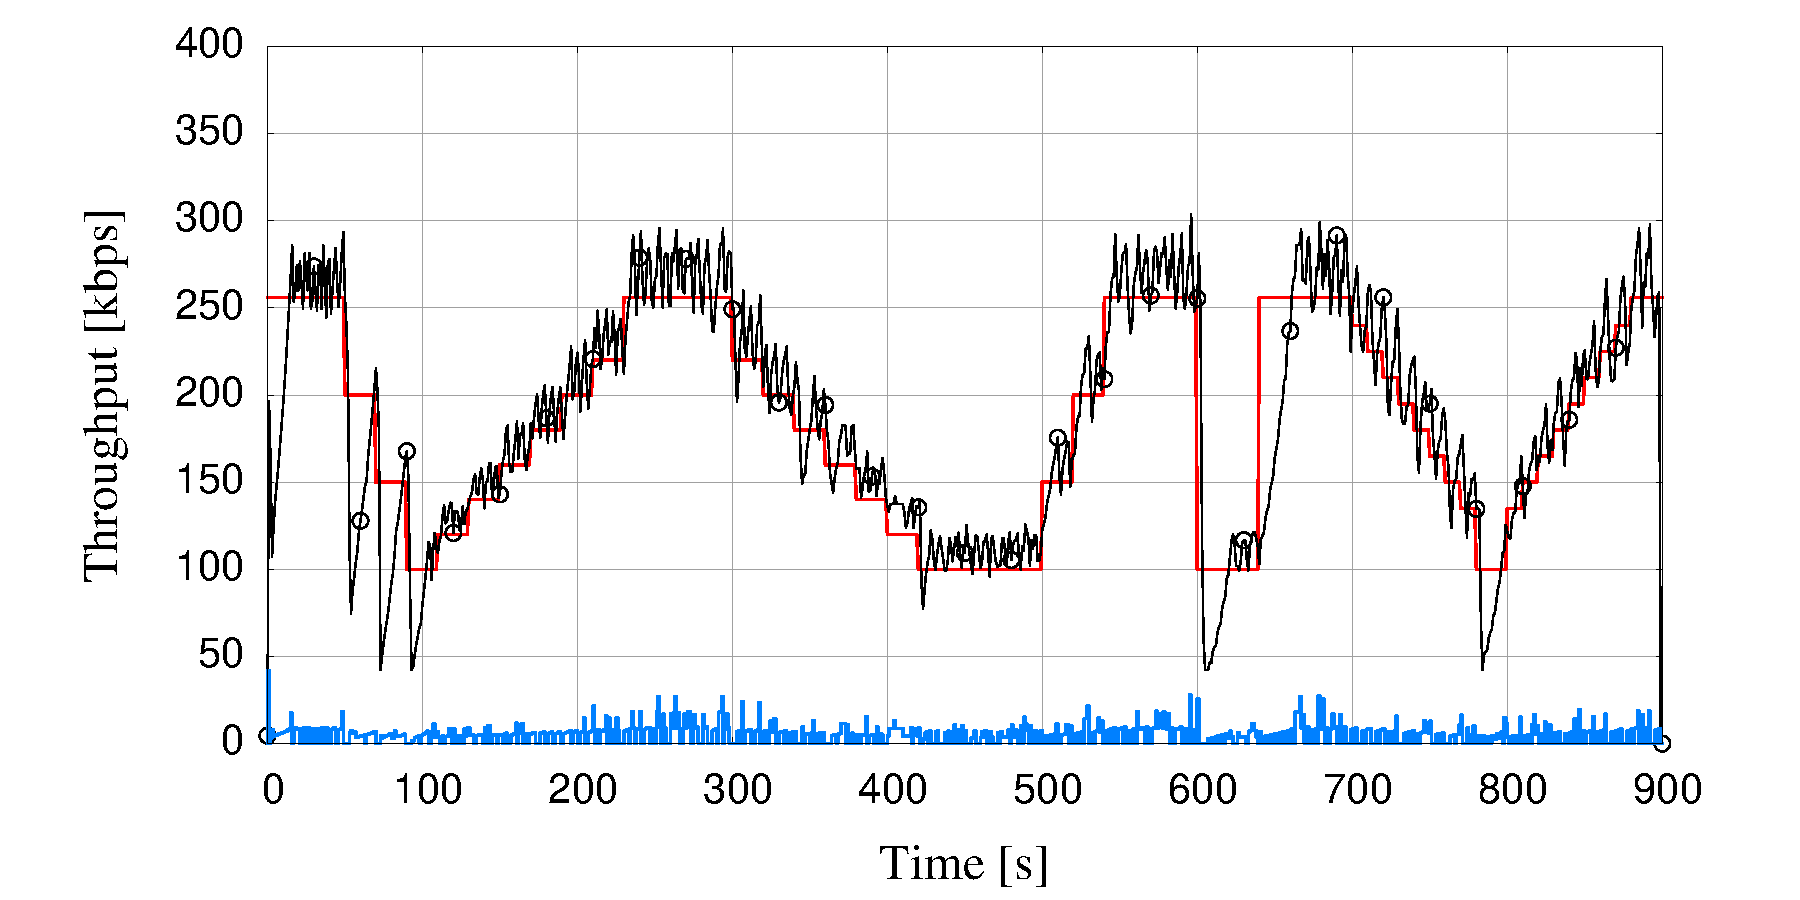
\includegraphics[width=0.5\textwidth]{chap6-graph-fecrc-var-50ms-2}
  } 
  \subfloat [OWD=100ms]{
    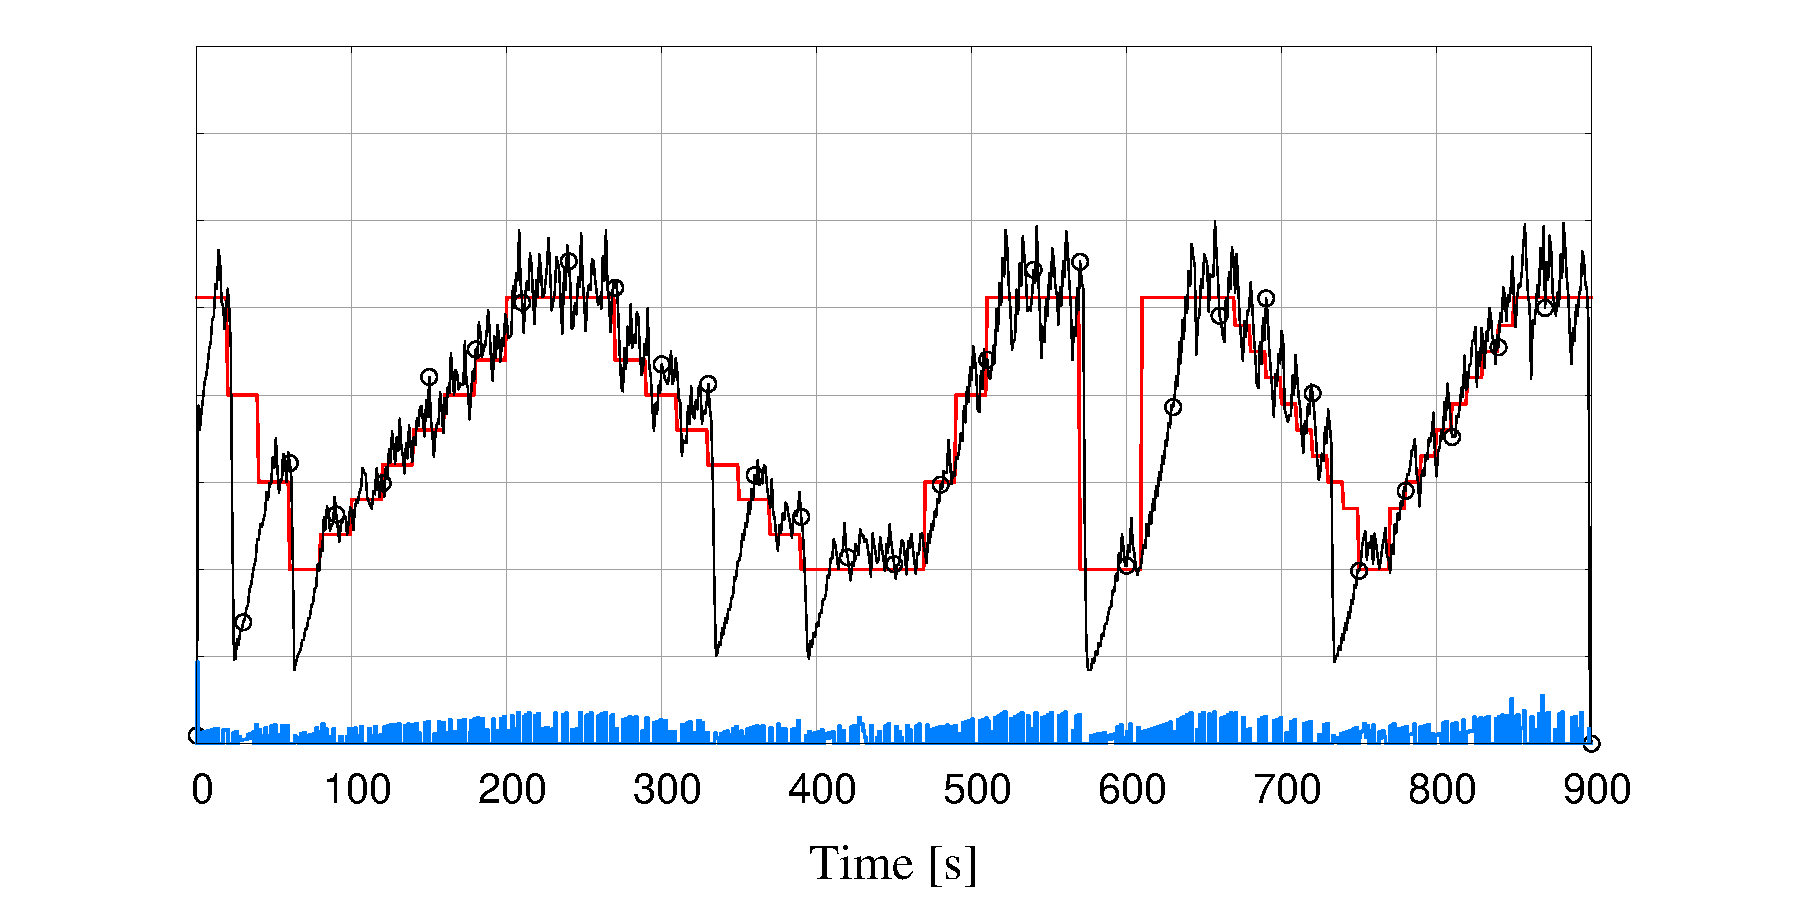
\includegraphics[width=0.5\textwidth]{chap6-graph-fecrc-var-100ms-2}
  } \\
  \subfloat [OWD = 240ms]{
    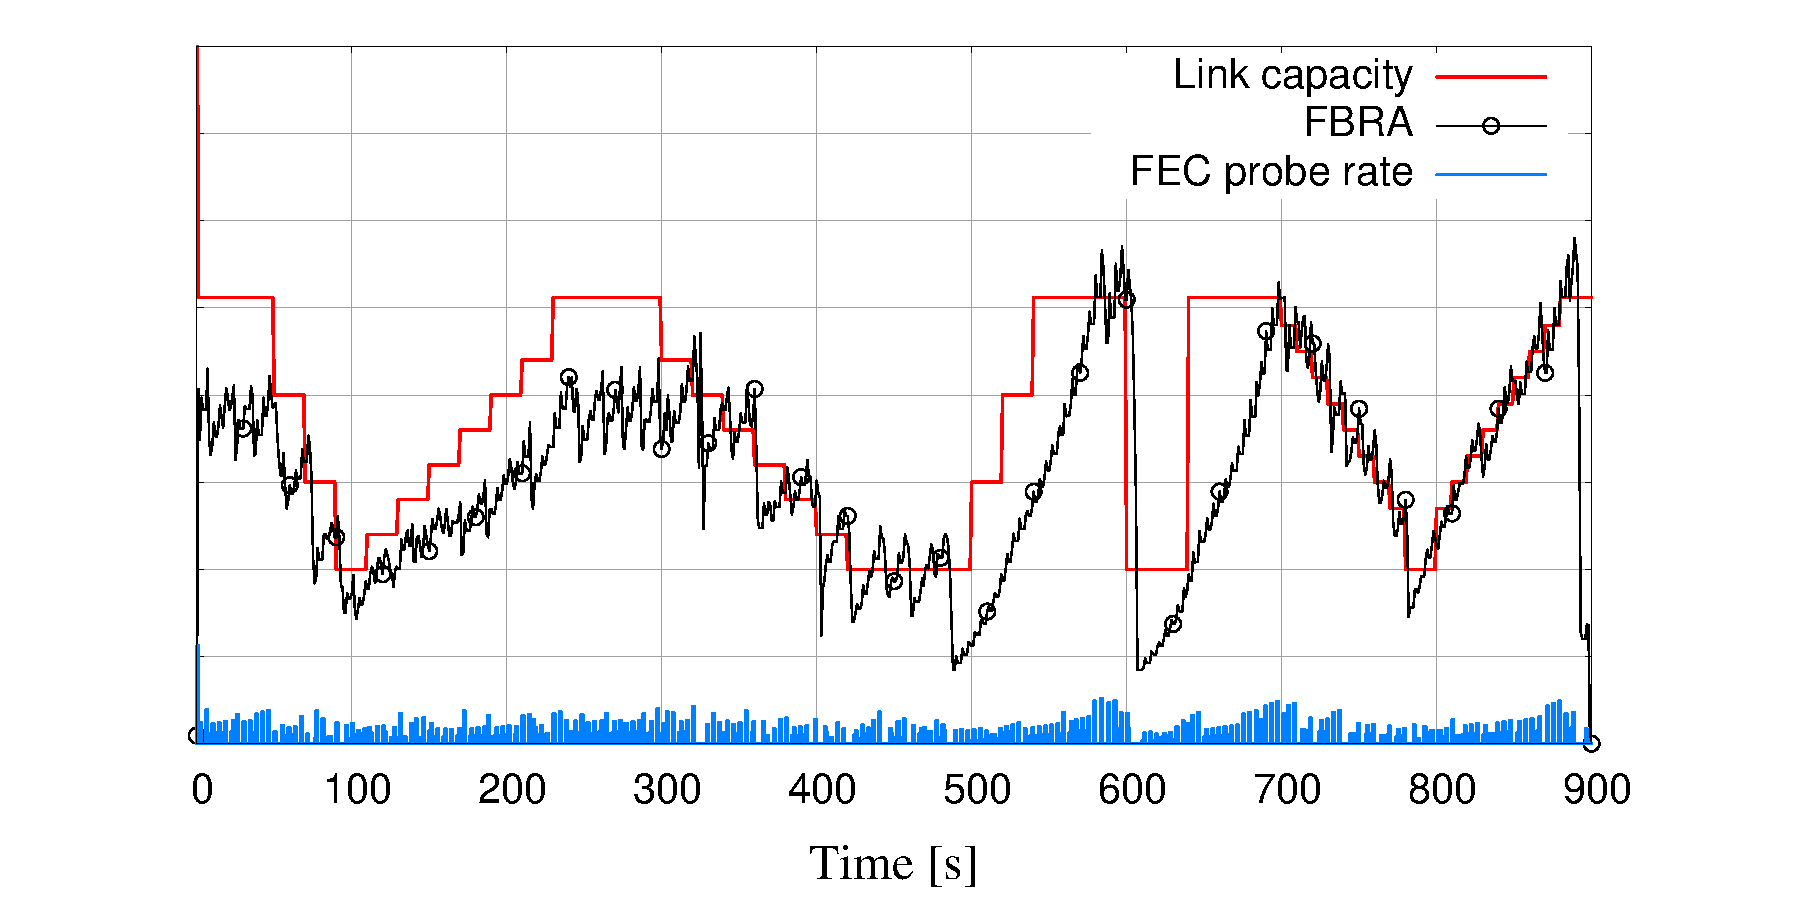
\includegraphics[width=0.5\textwidth]{chap6-graph-fecrc-var-240ms-2}
  }
}
\caption{Performance of a single RTP flow using FBRA in a
varying link capacity scenario with different bottleneck latencies. The plots
also show the FEC probing rate. We observe that the FEC rate is low when the
FBRA rate drops and FEC rate is high when the FBRA is ramping-up.}
\label{fig:fecrc-var}
\end{figure}

In \citepub{c:fecrc}, we compare the performance of FEC-Based Rate Adaptation
(FBRA), RRTCC and C-NADU. The bottleneck link capacity varies between
100\,\emph{kbps} and 256\,\emph{kbps}. In the scenario, we evaluate the
reactivity and convergence of the rate-control algorithm to the available 
end-to-end capacity for different path latencies. Our simulations in
\emph{ns-2}~\cite{ns2} shows that, for the 50\,\emph{ms} and 100\,\emph{ms}
bottleneck link latency, the goodput achieved by FBRA is comparable to RRTCC
but with comparatively lower loss rates ($\approx$1.5\,\%, see
Table~\ref{table:fecrc-var-res}). Figures~\ref{fig:fecrc-var}(a)--(b) show
that the FBRA can quite quickly bounce-back after undershooting. The figure
also shows that the FEC probing rate increases when the FBRA ramps up and the
FEC rate is low or disabled when the FBRA undershoots. However, FBRA is
primarily a delay-based control algorithm, and for the 240\emph{ms} bottleneck
delay, it observes that the packets are arriving very close to the 
application-defined maximum delay ($\approx$400ms) and is therefore, conservative in its
probing for available bandwidth (this is observed by the low FEC rate in
Figure~\ref{fig:fecrc-var}(c)). The FEC rate is about 10\,\% of the media rate at
about 15-20\,\emph{kbps} and the packet loss recovery is around 30\,\%.
Compared to FBRA, RRTCC tries to achieve high throughput at the cost of
incurring packet losses (this behavior is also observed in \ref{tab:rrtcc-loss}), 
while C-NADU trades off packet loss for throughput. In our
experiments, FBRA's performance is placed between the two trade-offs: better
throughput than C-NADU and lower loss ratio than RRTCC.


\begin{table}
  \centering{
  \scalebox{0.75}{
  \begin{tabular}{c c c c c}
  \hline
  \multirow{2}{*}{\textbf{Delay}} & \multirow{2}{*}{\textbf{Metric}} & \textbf{FBRA} & \textbf{RRTCC} & \textbf{C-NADU} \\ \cline{3-5}
  & & avg. $\pm\sigma$ & avg. $\pm\sigma$ & avg. $\pm\sigma$ \\ \hline
  \multirow{3}{*}{\begin{sideways} 50ms \end{sideways}} & Goodput [kbps] & 179.13 $\pm$2.26 &181.8 $\pm$3.11& 165.42 $\pm$3.87 \\ %\cline{2-8}
  & Loss rate [\%] & 1.23 $\pm$0.28 & 4.27 $\pm$0.78 & 0.34 $\pm$0.11\\ %\cline{2-8}
  %& \textbf{FEC rate [kbps]} & 17.51 & 1.18 & - & -& -& -\\ \cline{2-8}
  & No. of lost frames & 441.43 $\pm$82.37 & 1842 $\pm$25.4&93.67 $\pm$29.64 \\ \hline
  %& \textbf{No. of FEC protected lost frames} & 91.37 & 36.55 & - & -& -& - \\ \cline{2-8}
  %&\textbf{FRCC[\%]}& 92.57 & 2.84 & - & -& -& - \\ \hline
  \multirow{3}{*}{\begin{sideways} 100ms \end{sideways}} & Goodput [kbps] & 172.83 $\pm$2.74 & 172.48 $\pm$6.6 & 163.84 $\pm$3.11\\ %\cline{2-8}
  & Loss rate [\%] & 1.72 $\pm$0.37 & 3.09 $\pm$0.85 & 0.17 $\pm$0.09\\ %\cline{2-8}
  %& \textbf{FEC rate [kbps]} & 20.05 & 1.34 & - & -& -& - \\ \cline{2-8}
  & No. of lost frames & 562.83 $\pm$103.44 & 740 $\pm$42.82& 46.4 $\pm$22.94\\ \hline
  %& \textbf{No. of FEC protected lost frames} & 130.57 & 45.41 & - & -& -& - \\ \cline{2-8}
  %& \textbf{FRCC[\%]} & 95.85 & 1.95 & - & -& -& - \\ \hline
  \multirow{3}{*}{\begin{sideways} 240ms \end{sideways}} &Goodput [kbps] & 144.89 $\pm$8.35 & 169.22 $\pm$5.68 & 153.52 $\pm$6.81\\ %\cline{2-8}
  & Loss rate [\%] & 2.82 $\pm$0.89 & 2.98 $\pm$0.55&0.19 $\pm$0.07 \\ %\cline{2-8}
  %& \textbf{FEC rate [kbps]} & 16.22 & 0.56 & - & -& -& - \\ \cline{2-8}
  & No. of lost frames & 789.93 $\pm$223.55 & 705.67 $\pm$41.33 & 53.23  $\pm$21.41 \\ \hline
  %& \textbf{No. of FEC protected lost frames} & 178.07 & 69.92 & - & -& -& - \\ \cline{2-8}
  %& \textbf{FRCC[\%]} & 90.1 & 7.26 & - & -& -& - \\ \hline
  \end{tabular}
  }}
  \caption{Overall metrics for an RTP flow on a variable capacity link.
  Results are the average of 30 runs.}
  \label{table:fecrc-var-res}
\end{table}


% RRTCC achieves the best goodput ($169$-$180 kbps$) for the three bottleneck
% link latencies, but has the worst loss rate ($3$-$4\%$). RRTCC is aggressive
% in its probing for available bandwidth and does not react to losses up to
% $2\%$. On the other hand, C-NADU achieves excellent reliability
% ($0.15$-$0.5\%$) results in all the cases, but observes lower goodput (about
% $10$-$15kbps$ lower than RRTCC). The two algorithms trade-off throughput for
% packet loss and vice-versa.

% Table of FEC, C-NADU and RRTCC :)


\begin{table}
  % \resizebox{\textwidth}{!}{%
  \centering{
  \scalebox{0.75}{
  \begin{tabular}{cccc}
  \hline
  \multirow{2}{*}{\textbf{Delay}} & \multirow{2}{*}{\textbf{Metric}} & \textbf{Call 1} & \textbf{Call 2} \\ \cline{3-4}
  & & avg. $\pm \sigma$ & avg. $\pm \sigma$ \\ \hline 
  \multirow{5}{*}{\begin{sideways} 50ms \end{sideways}} 
  & Goodput [kb/s] & 375.39 $\pm$ 88.25 & 348.77 $\pm$ 83.64 \\ 
  & Loss rate [\%] & 1.21 $\pm$ 0.19 & 1.39 $\pm$ 0.69 \\ 
  & FEC rate [kb/s] & 12.24 $\pm$ 1.64 & 11.78 $\pm$ 1.39 \\ 
  & No. of FEC protected lost frames & 15.3 $\pm$ 3.44 & 14.6 $\pm$ 2.73 \\ 
  & No. of recovered frames & 7.4 $\pm$ 2.83 & 6.9 $\pm$ 3.33 \\ 
  & PSNR [dB] & 38.08 $\pm$ 2.1 & 37.7 $\pm$ 1.53 \\ \hline
  %& \textbf{Lossless PSNR [dB]} &  &  &  &  \\ \hline 
  \multirow{5}{*}{\begin{sideways} 100ms \end{sideways}} 
  & Goodput [kb/s] & 295.33 $\pm$ 48.27 & 351.1 $\pm$ 63.4 \\ 
  & Loss rate [\%] & 3.15 $\pm$ 0.93 & 2.33 $\pm$ 0.87 \\ 
  & FEC rate [kb/s] & 10.7 $\pm$ 0.68 & 11.69 $\pm$ 1.52 \\ 
  & No. of FEC protected lost frames & 3.0 $\pm$ 2.1 & 4.1 $\pm$ 3.14 \\ 
  & No. of recovered frames & 7.3 $\pm$ 3.03 & 4.5 $\pm$ 3.07 \\ 
  & PSNR [dB] & 35.64 $\pm$ 1.17 & 37.32 $\pm$ 1.65 \\ \hline
  %& \textbf{Lossless PSNR [dB]} & & & & \\ \hline 
  \end{tabular}
  }}
  \caption{Two FBRA flows on a bottleneck link in an emulated testbed. Results
  are the average of 10 runs.}
  \label{table:fecrc-rw-udp}
\end{table}

In \citepub{c:fecrc}, we also measure the performance of two FBRA calls
competing on a bottleneck link (1\,\emph{Mbps}) in a testbed. The difference in the
goodput of the calls in the two latency scenarios (50\,\emph{ms} and
100\,\emph{ms}) is about 30-50\,\emph{Kbps}, but the PSNR of these calls is
similar (see Table~\ref{table:fecrc-rw-udp}). Therefore, as far as we can tell from
PSNR, the small rate variations have little bearing on the quality of the
call. The FEC recovery is low due to the small amount of packet loss, and most of
the losses occur when FEC was disabled. Additionally, 90\,\% of the times FEC
was enabled resulted in an increase in media rate. Low FEC overhead also
implies that the FBRA remains longer in the \texttt{\emph{STAY}} state, thus
avoiding abrupt changes to the encoding rate, which is detrimental for user
experience \cite{Zink03subjectiveimpression}.

\begin{table}
  % \resizebox{\textwidth}{!}{%
  \centering{
  \scalebox{0.75}{
  \begin{tabular}{ccc}
  \hline
  \textbf{Metric} & \textbf{50ms delay} & \textbf{100ms delay} \\ \cline{2-3}
  & avg. $\pm\,\sigma$ & avg. $\pm\,\sigma$ \\ \hline 
  Goodput [kb/s] & 302.24 $\pm$ 87.07 & 280.97 $\pm$ 92.15 \\
  Loss rate [\%] & 4.24 $\pm$ 0.89 & 4.1 $\pm$ 0.58 \\
  FEC rate [kb/s] & 13.6 $\pm$ 2.15 & 12.58 $\pm$ 2.18 \\
  No. of lost frames & 154.6 $\pm$ 16.56 & 170.9 $\pm$ 12.38 \\
  No. of FEC protected lost frames & 38.0 $\pm$ 6.08 & 23.7 $\pm$ 8.99 \\ 
  No. of recovered frames & 7.4 $\pm$ 2.83 & 6.9 $\pm$ 3.33 \\
  PSNR [dB] & 35.62 $\pm$ 1.49 & 34.7 $\pm$ 2.26 \\
  TCP throughput [kbit/s] & 612.22 $\pm$ 48.45 & 575.11 $\pm$ 45.67 \\ \hline
  %\textbf{Lossless PSNR [dB]} &  &  &  &  \\ \hline 
  \end{tabular}
  }}
  \caption{An RTP flow sharing a bottleneck link with short TCP flows in an
  emulated testbed. Results are average of 10 runs.}
  \label{table:fecrc-rw-tcp}
\end{table}


When competing with short TCP flows, the FBRA achieves an average goodput of
302\,\emph{kbps} and 280\,\emph{kbps} in the 50\,\emph{ms} and 100\,\emph{ms}
latency scenario, respectively (see Table~\ref{table:fecrc-rw-tcp}).
Additionally, about 85\,\% of the times FEC was enabled, resulted in an
increase in media rate. The TCP flow achieves a throughput of around
600\,\emph{kbps} on average. The PSNR in both scenarios are very similar
($\approx$ 35dB), but the PSNR is lower for the 100\,\emph{ms} delay scenario because the
average goodput is also a bit lower in this case (see Figure~\ref{fig:fecrc-dnet}).


\begin{figure}
  \centering{
  \subfloat [50ms]{
    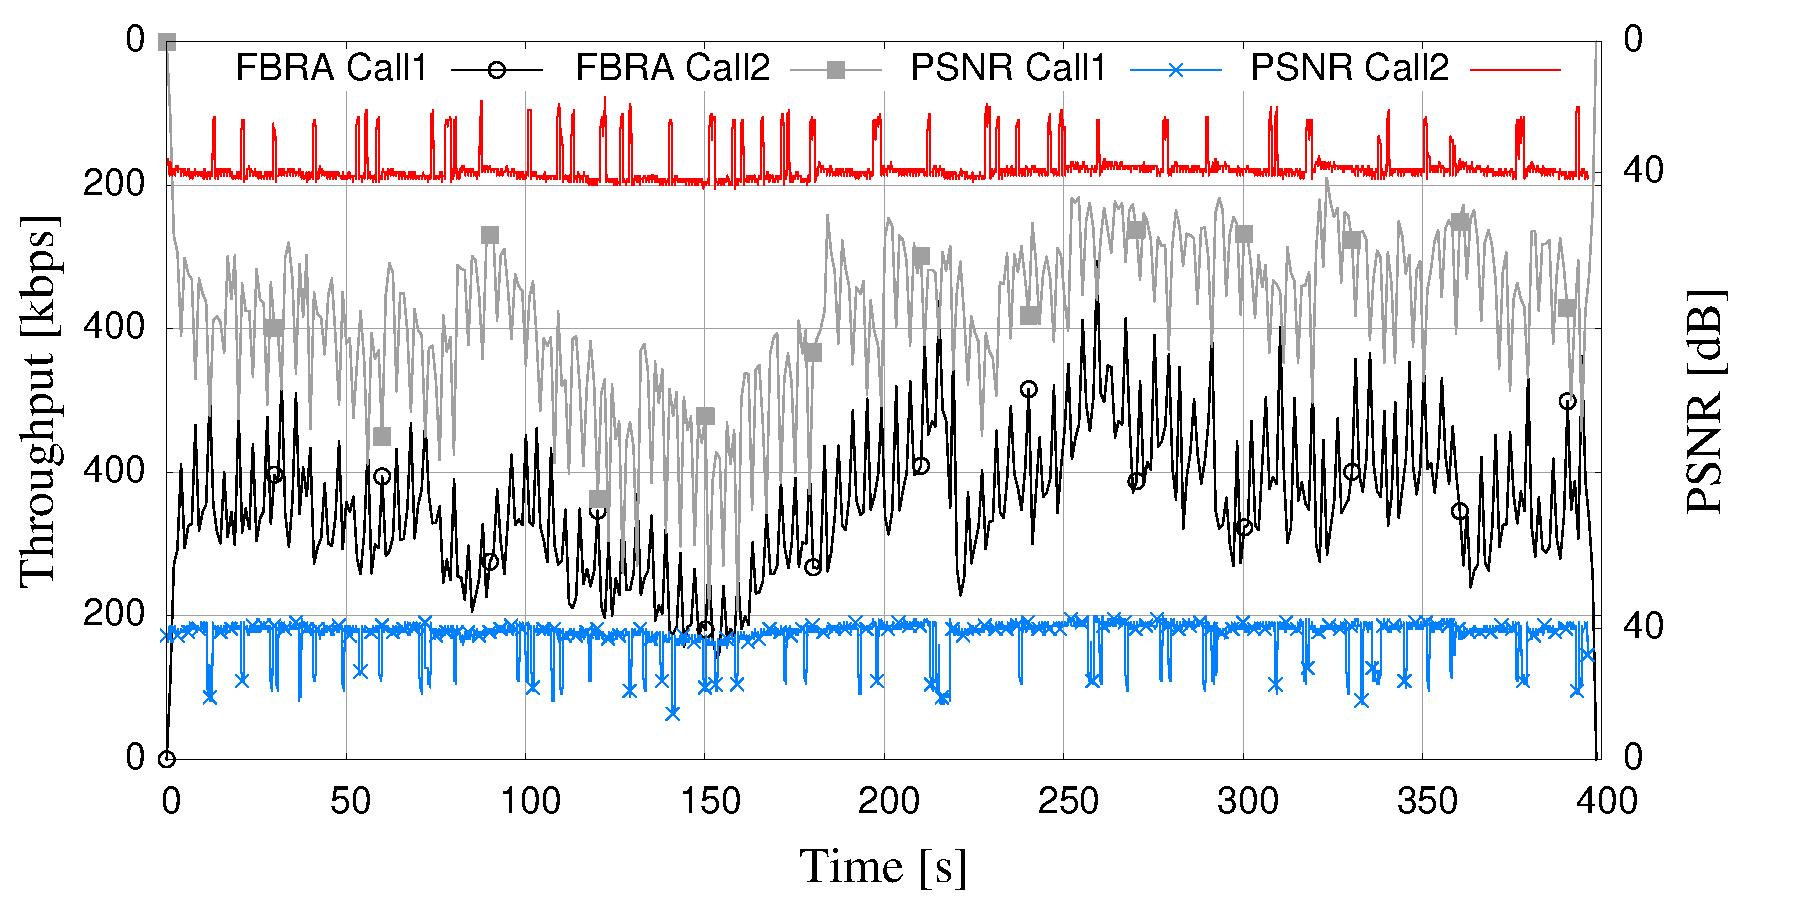
\includegraphics[width=0.66\textwidth]{chap6-graph-fecrc-dummynet-50ms-2}
  } \\
  \subfloat [100ms]{
    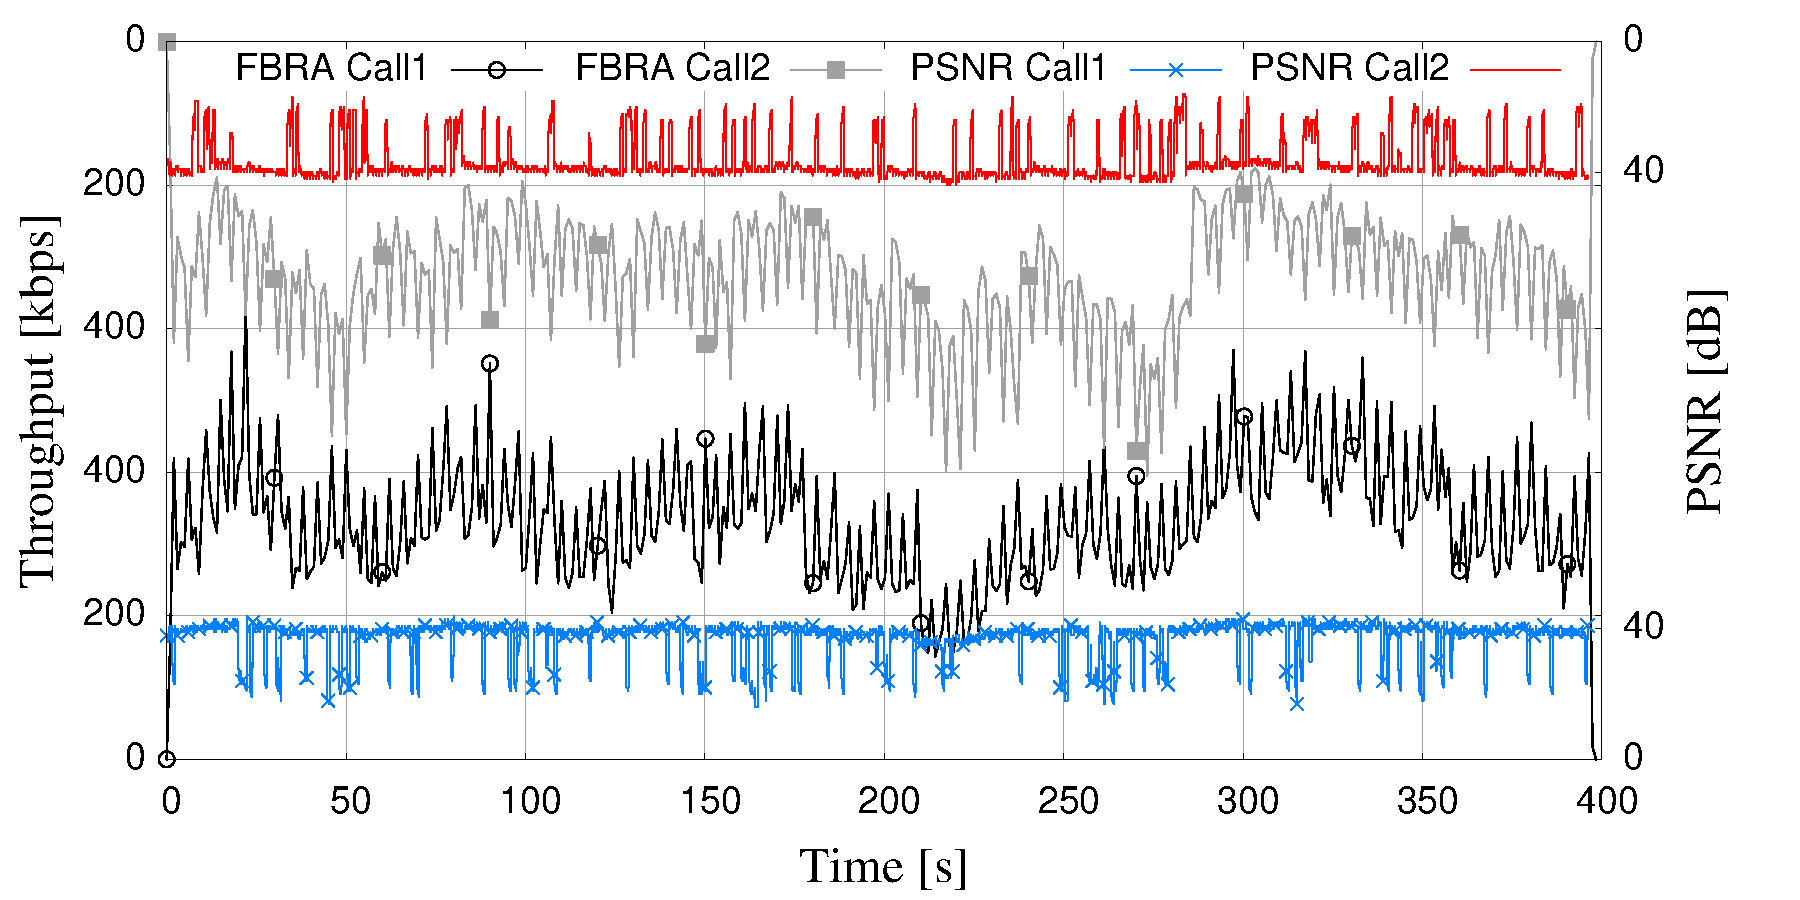
\includegraphics[width=0.66\textwidth]{chap6-graph-fecrc-dummynet-100ms-2}
  }
}
\caption{The plots show the goodput of two RTP calls sharing a common
bottleneck. To illustrate amount of empty link capacity and how two flows push
one another, we plot one of them on the reverse axis. The end-to-end path
capacity is \emph{1 Mbps} in both delay scenarios and delays are \emph{50ms}
and \emph{100ms}. The plot also shows the PSNR variation for the two calls (on
the minor Y-axis).}
\label{fig:fecrc-dnet}
\end{figure}

% Lastly, we measure the performance of the FBRA on the public Internet, between
% a host on Amazon EC2 instance in Ireland and a machine at Aalto University. We
% observe varying results between each successive run, as the public Internet
% has varying amount of cross traffic. The goodput ranges between $100$-$700$
% \emph{kbps}, the maximum loss rate does not exceed $1.5\%$, the PSNR of the
% calls varies between $35$-$40$ \emph{dB}. Despite the diversity in results, it
% show that FBRA may work in the public Internet.

\section{Summary}

In this chapter, we address two problems: applicability of error-resilience
schemes and the use of FEC to probe for available capacity in a multimedia congestion
control algorithm. In the first case, we show that NACK, RPS, UEP/FEC and adaptive 
slice-size can be used for different levels of latencies and observed packet
loss ratio. We also observed that sending smaller packets in mobile networks
performed better than sending MTU-sized ($\approx$ 1500 bytes) packets.
Alternatively, the MTU sized packets were better suited for wired or fixed
networks where bit errors occurred less often.

In the second case, we propose a congestion control scheme where instead of
increasing the rate when network conditions seem stable, the sender introduces
FEC for one RTCP interval. If the FEC and the media packets are received
successfully, sender rate increases by the amount of the FEC rate. 
The trade-off is that we get a smoother ramp-up and, if a packet gets
lost, it may be recovered by the FEC packet. The sender also implements a
variable FEC interval, i.e., it varies the number of packets for which FEC is
generated. Hence, if the sender thinks that it is under utilizing the link by a
large margin, it introduces a shorter FEC interval (up to 33\,\% redundancy)
and therefore ramps up quickly. Consequently, when the sender thinks that it is closer
to the bottleneck link capacity, it introduces a longer FEC interval (up to
8\,\% redundancy) and therefore is conservative in probing for available
capacity. Our experiments show that by using adaptive FEC for probing, the
endpoints are able to recover 15-25\,\% of the lost packets, and,
$\approx$90\,\% of the time, using FEC subsequently results in an increase in
the media rate. These results are comparable to our earlier experiments using
a fixed FEC interval for error-resilience, where we were able to recover
20-24\;\% of the lost packets. We believe using FEC for congestion control in
interactive multimedia has not been explored in depth by the community, partly
because interactive multimedia flows have very tight delay constraints and FEC
may not arrive in time for recovering the packet.

This chapter concludes the discussion of congestion control based on 
\emph{in-path} sources and \emph{in-band} signaling. In the next two chapters, we will
discuss the use of congestion cues from off-path sources to perform congestion
control.
